\documentclass[9pt, twocolumn]{extarticle}
\setlength{\columnsep}{30px}
\usepackage[a4paper, margin=1.5cm, bmargin=2cm]{geometry}
\usepackage[hidelinks]{hyperref}
\usepackage{tcolorbox}
\usepackage{amssymb}
\usepackage{graphicx}
\usepackage{amsmath}
\usepackage{titlecaps}

\newtcolorbox{definitionbox}[2][]{
  colback=yellow!10!white,  % Background color
  colframe=yellow!50!black, % Border color
  fonttitle=\bfseries\itshape, % Title font style
  title={#2},
  #1 % Optional parameters from the user
}

\newcommand{\definition}[2]{%
  \begin{definitionbox}{\titlecap{#1}}
    #2
  \end{definitionbox}
}


\title{FTP\_TheoComp Summary}
\author{Valentin Huber\\\href{https://valentinhuber.me}{valentinhuber.me}}
\begin{document}
\maketitle
% \tableofcontents
\vspace{4em}

\definition{\NoCaseChange{iif}}{if and only if}

\section{Elementary Definitions}
\definition{Alphabet}{A finite set of symbols such as letters, digits, etc.}
Examples:
\begin{itemize}
  \item $\Sigma_1 = \{a,b,c\}$
  \item $\Sigma_2 = \{a,b,c,\ldots,z\}$
\end{itemize}

\definition{Word}{A word over an alphabet $\Sigma$ is a string of finite length, in other words a finite sequence of symbols of $\Sigma$}
\definition{Language}{A (formal) language over an alphabet $\Sigma$ is defined as a set of words (defined over $\Sigma$).}

The letters $w$, $u$, and $v$ are usually used for words, $s$, $t$, and $r$ for single characters. Languages are usually denoted by capital letters. Examples (over $\Sigma = \{a,b,c\}$):
\begin{itemize}
  \item $L_1 = \{a,~b,~aab,~abbcc\}$, a finite language
  \item $L_2 = \{acbb,~accbb,~acccbb,~accccbb,~\ldots\}$, words starting with $a$, then $n > 0$ $c$s and finally $bb$
\end{itemize}

We only consider finite alphabets, otherwise important and useful properties are no longer valid. A language can be infinite, but each element (i.e. word) is finite.

\subsection{Operations on Words}

\definition{Word Concatenation}{Appending the second word to the end of the first one, denoted by either $w_1\cdot w_2$, or simply $w_1w_2$}
\definition{Empty string}{$\epsilon$, where $|\epsilon| = 0$ and $w\cdot\epsilon=\epsilon\cdot w = w$}
\definition{Operations on Words}{
  \begin{itemize}
    \item Word length: Number of symbols in a word, denoted as $|w|$
    \item Mirror (reverse): $w=s_1s_2\ldots s_n\Rightarrow w^R=s_n\ldots s_2s_1$
    \item Palindrome: if $w=w^R$, e.g. $sugus$
    \item Concatenation with self: $w^n, n\ge0$, concat of $w$ with itself $n$ times
  \end{itemize}

}

\definition{Set of all words}{$\Sigma^+$ is the set of all words $w$ with $|w|>0$ over $\Sigma$, $\Sigma^* = \Sigma^+ \cup \{\epsilon\}$}
$\Sigma^+$ and $\Sigma^*$ are infinite iif $\Sigma\neq\varnothing$

\subsection{Operations on Languages}

\definition{Language-Operations}{
  Union: $L_1\cup L_2$

  Intersection: $L_1\cap L_2$

  Complement: $\overline{L}=\Sigma^*\backslash L$

  Concatenation: $L_1\cdot L_2=\{w_1\cdot w_2 | w_1\in L_1, w_2\in L_2\}$

  Neutral Element: $L_\epsilon = \{\epsilon\} (L\cdot L_\epsilon = L_\epsilon\cdot L = L)$

  Absorbant Element: $\varnothing (L\cdot\varnothing=\varnothing\cdot L=\varnothing\neq L_\epsilon)$

  Self-Concatenation: $L^n, n\ge0$, $(L^0=L_\epsilon = \{\epsilon\})$
}

\definition{Iterative or Kleene's Closure}{$L^*$, is the set of words resulting of the concatenation of a finite number of words of $L$, where $$L^+=L^1\cup L^2\cup L^3\ldots=\displaystyle\bigcup_{i\ge1}L^i=L\cdot L^*$$}

All words in a Kleene's closure have finite length. $\epsilon$ belongs to $L^*$, but not always to $L^+$ ($\varnothing^*=L^0=\{\epsilon\}$).

\section{Finite State Automata and Regular Languages}
\subsection{Finite State Automata (FSA)}
A FSA is equivalent to an oriented graph and composed of
\begin{itemize}
  \item  finite set of states (drawn as circles),
  \item  transition function describing the actions which allow to
        move from one state to another (these are the arrows), and
  \item the initial state in which the system is at the beginning (this
        state is indicated by an arrow pointing at it from nowhere).
\end{itemize}

\subsection{Deterministic FSA (DFA)}
\definition{Deterministic FSA (DFA)}{

  A DFA is a 4-tuple $\langle Q, \Sigma, \delta, q_0\rangle$ where
  \begin{itemize}
    \item $Q$ is a finite set of states (therefore \textbf{F}SA),
    \item $\Sigma$ is a finite set of symbols (alphabet),
    \item $\delta: Q \times \Sigma \rightarrow Q$ is a transition function,
    \item $q_0 \in Q$ is the initial state.
  \end{itemize}
}

The extension of $\delta$ is the function $\delta^*: Q \times \Sigma^* \rightarrow Q$ which provides the next state for a sequence of symbols.

\definition{Extension of Transition Function} {
  For a state $q \in Q$, a word $w \in \Sigma^*$, and a symbol $s \in \Sigma$, the function $\delta^*: Q \times \Sigma^* \rightarrow Q$ is recursively defined as follows:
  \begin{enumerate}
    \item $\delta^*(q, \epsilon)=q$,
    \item $\delta^*(q, w s)=\delta(\delta^*(q, w), s)$.
  \end{enumerate}
}
The sequence of symbols is actually a word.

\definition{DFA language recognizer}{
  A DFA together with a set of final states $F\subseteq Q$, drawn as double circles.

  A word $w\in\Sigma^*$ is recognized by a DFA of $\langle Q,\Sigma, \delta, q_0, F\rangle$ iif $\delta^*(q_0,w)\in F$

  $L(M)$ is the language as recognized by such a language recognizer.
}

\definition{Regular Language}{Every language recognized by a finite state recognizer automaton.}

\subsection{Non-deterministic Finite Automata (NFA)}

\definition{Non-deterministic Finite State Automaton (NFA)}{
  A NFA is a 5-tuple $\langle Q, \Sigma, \delta, q_0, F \rangle$ similar to a DFA, except the transition function $\delta$ is defined as $Q \times \Sigma \rightarrow \mathcal{P}(Q)$ where $\mathcal{P}(Q)$ is the power function of $Q$.
}


\definition{Extension of Transition Function for NFA} {
  For a state $q \in Q$, a word $w \in \Sigma^*$, and a symbol $s \in \Sigma$, the function $\delta^*: Q \times \Sigma^* \rightarrow \mathcal{P}(Q)$ is defined as follows:
  \begin{enumerate}
    \item $\delta^*(q, \epsilon)=\{q\}$,
    \item $\delta^*(q, ws)= \displaystyle\bigcup_{q' \in \delta^*(q, w)} \delta(q', s)$.
  \end{enumerate}
}
This means that for a word $ws$, the set of possible states is obtained by applying the transition function $\delta$ to all states reached by $\delta^*(q, w)$ with symbol $s$ and taking the union of all resulting states.

\definition{Extension of Transition Function to $\mathcal{P}(Q)$}{
  $$\begin{aligned}
      \delta: \mathcal{P}(Q) \times \Sigma     & \rightarrow \mathcal{P}(Q)               \\
      (P, s)                                   & \mapsto  \bigcup_{p \in P} \delta(p, s)  \\
      \delta^*: \mathcal{P}(Q) \times \Sigma^* & \rightarrow \mathcal{P}(Q)               \\
      (P, w)                                   & \mapsto \bigcup_{p \in P} \delta^*(p, w)
    \end{aligned}$$
}

\subsubsection{Equivalence of DFA and NFA}

\definition{Equivalence of Automata} {
  Two finite state automata $M_1$ and $M_2$ are equivalent if and only if they recognize the same language, i.e., $L(M_1) = L(M_2)$.
}

\paragraph{Construction of DFA from NFA}
Let $M = \langle Q, \Sigma, \delta, q_0, F \rangle$ be a NFA. We construct a DFA $M' = \langle Q', \Sigma, \delta', q_0', F' \rangle$ as follows:
\begin{itemize}
  \item $Q' = \mathcal{P}(Q)$, the power set of $Q$, where an element of $Q'$ will be denoted $[q_1,q_2,\ldots,q_i]$,
  \item $q_0' = \{q_0\}$,
  \item $F' = \{S \subseteq Q \mid S \cap F \neq \varnothing\}$, the set of members of $Q'$ composed of at least one final state $M$,
  \item $\delta' : Q' \times \Sigma \rightarrow Q'$ with $\delta'(S, a) = \displaystyle\bigcup_{q \in S} \delta(q, a)$, so $\delta'([q_1,\ldots,q_i],s)=[p_1,\ldots,p_j] \Longleftrightarrow \delta(\{q_1,\ldots, q_i\},s)=\{p_1\ldots,p_j\}$.
\end{itemize}

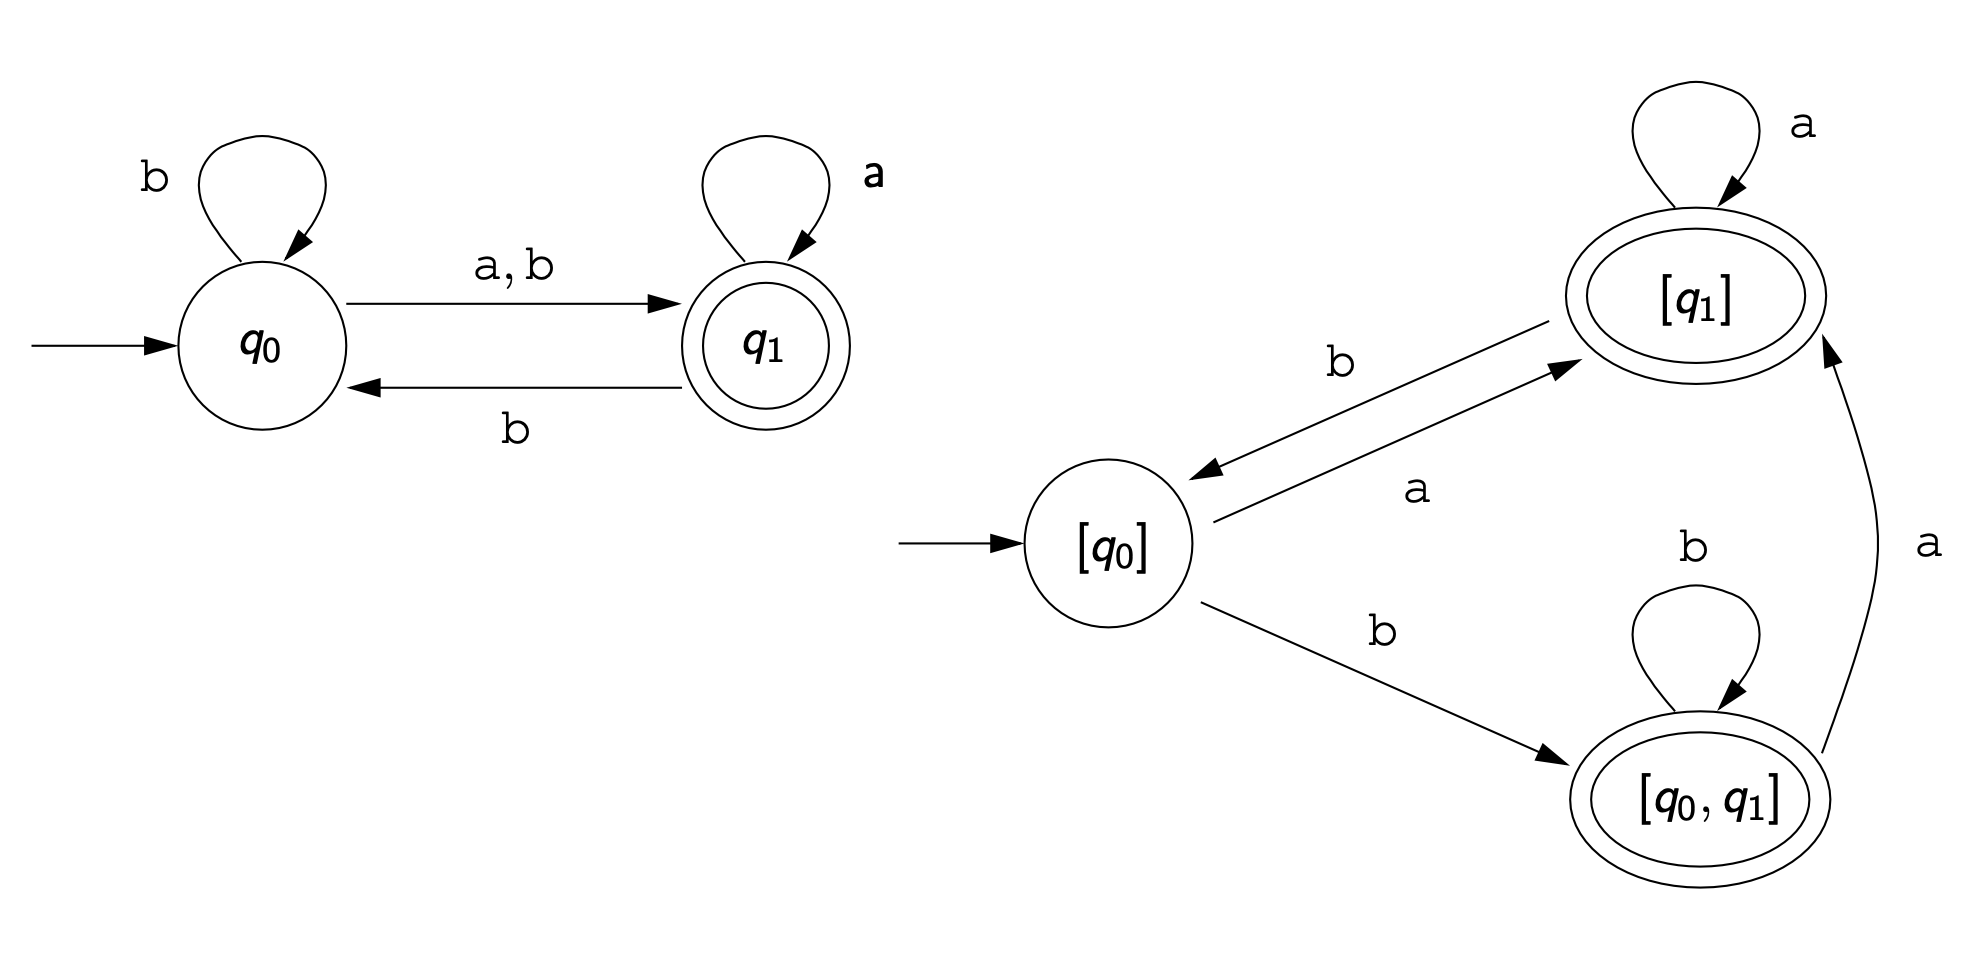
\includegraphics[width=0.95\columnwidth]{assets/NFA-DFA.png}

\paragraph{Proof}
We prove by induction on the length of $w$ that for any $w \in \Sigma^*$:
\[ \delta'^*(q_0', w) = \delta^*(q_0, w) \]

Base Case: For $w = \epsilon$, $\delta'^*(q_0', \epsilon) = q_0' = \{q_0\}$ and $\delta^*(q_0, \epsilon) = \{q_0\}$.

Induction Step:
Let us assume that the above expression is true for some words of length $\leq m$. Let $s \in \Sigma$ and $w s$ be a string of length $m+1$. By definition of $\delta'^*$
$$
  \delta'^*(q_0^{\prime}, w s)=\delta^{\prime}(\delta'^*(q_0^{\prime}, w), s)
$$

By induction hypothesis,
$$
  \delta'^*(q_0^{\prime}, w)=[p_1, \ldots, p_j] \Longleftrightarrow \delta^*(q_0, w)=\{p_1, \ldots, p_j\} .
$$

But, by definition of $\delta^{\prime}$,
$$\begin{aligned}
                             & \delta^{\prime}([p_1, \ldots, p_j], s)=[r_1, \ldots, r_k] \\
    \Longleftrightarrow\quad & \delta(\{p_1, \ldots, p_j\}, s)=\{r_1, \ldots, r_k\}
  \end{aligned}$$

Consequently,
$$
  \delta'^*(q_0^{\prime}, w s)=[r_1, \ldots, r_k] \Longleftrightarrow \delta^*(q_0, w s)=\{r_1, \ldots, r_k\} .
$$

Finally, we have to add the following $\delta'^*(q_0^{\prime}, w) \in F^{\prime}$ only when $\delta^*(q_0, w)$ contains a state of $Q$ that belongs to $F$. Thus, $L(M)=L(M^{\prime})$

\paragraph{Construction of DFA from NFA}
To convert a NFA $M = \langle Q, \Sigma, \delta, q_0, F \rangle$ to a DFA $M' = \langle Q', \Sigma, \delta', q_0', F' \rangle$:

\begin{itemize}
  \item $Q'$: Create a new set of states, which is the power set of $Q$ (all possible subsets of $Q$). Each state in the DFA represents a set of states in the NFA.
  \item $q_0'$: The initial state in the DFA is the set containing the initial state of the NFA, ${q_0}$.
  \item $F'$: The final states in the DFA are all sets of states in $Q'$ that include at least one final state from $F$.
  \item $\delta'$: Define the transition function for the DFA. For each set of states $S$ in $Q'$ and each input symbol $a \in \Sigma$ (start with $q_0$):
        \begin{enumerate}
          \item Compute $\delta(S, a)$ by finding the set of all possible states the NFA can transition to from any state in $S$ on input $a$.
          \item Formally, $\delta'(S, a) = \displaystyle\bigcup_{q \in S} \delta(q, a)$.
          \item Example: If $S = {q_1, q_2}$ and $\delta(q_1, a) = {q_3}$ and $\delta(q_2, a) = {q_4, q_5}$, then $\delta'({q_1, q_2}, a) = {q_3, q_4, q_5}$.
        \end{enumerate}
\end{itemize}



\subsection{\texorpdfstring{NFAs with $\epsilon$-Transitions}{NFAs with Epsilon-Transitions}}
\definition{Automaton with $\epsilon$-Transitions}{A finite state automaton with $\epsilon$-transition is defined in the same
  manner as a classic nondeterministic automata except that the symbol $\epsilon$ is in the alphabet}
\definition{$\epsilon$-Closure}{The set of all states of an automaton $M$ reachable from a state $q$ by a sequence of empty transitions}
\paragraph{Removing $\epsilon$-transitions}
Calculate $\delta^*$ as a table of rows correlating with each state and columns of each input and fields as sets of states. Maybe add $q_0$ if the empty string is recognized by the automaton.

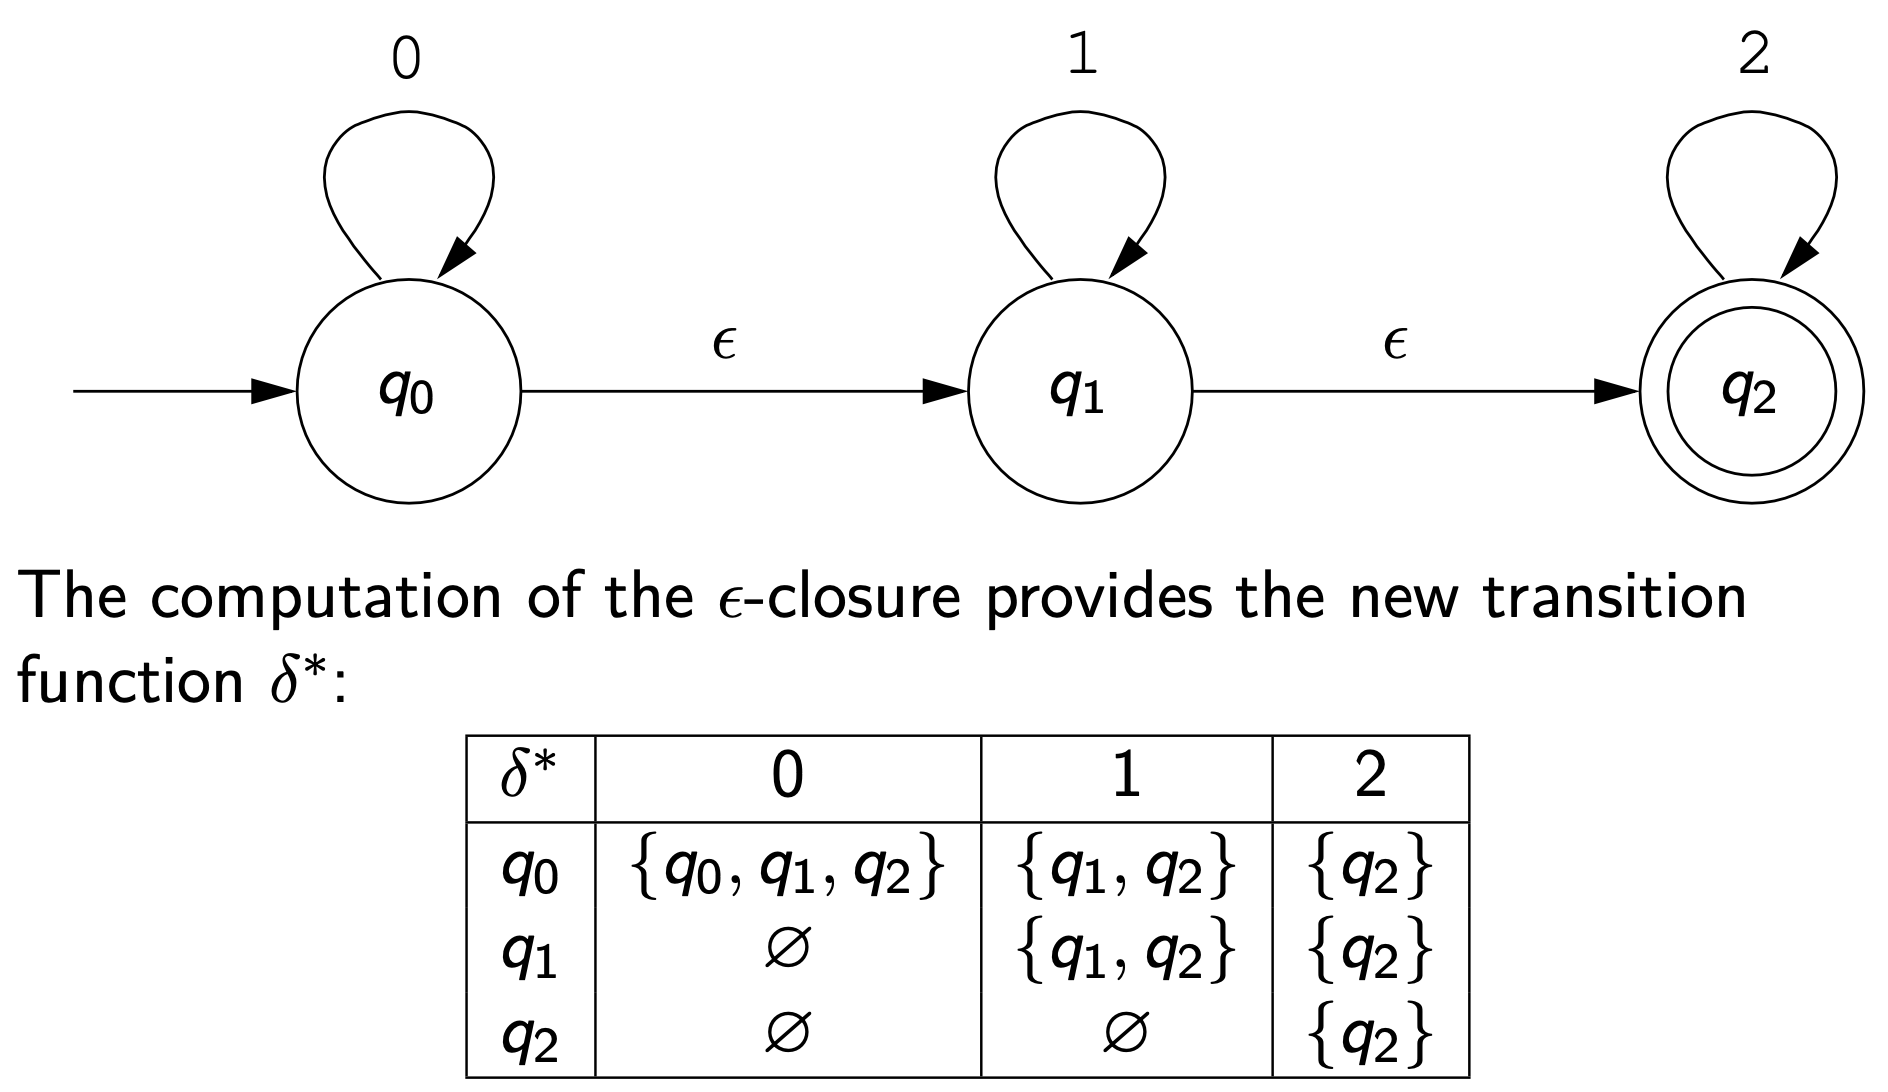
\includegraphics[width=0.95\columnwidth]{assets/epsilon1.png}
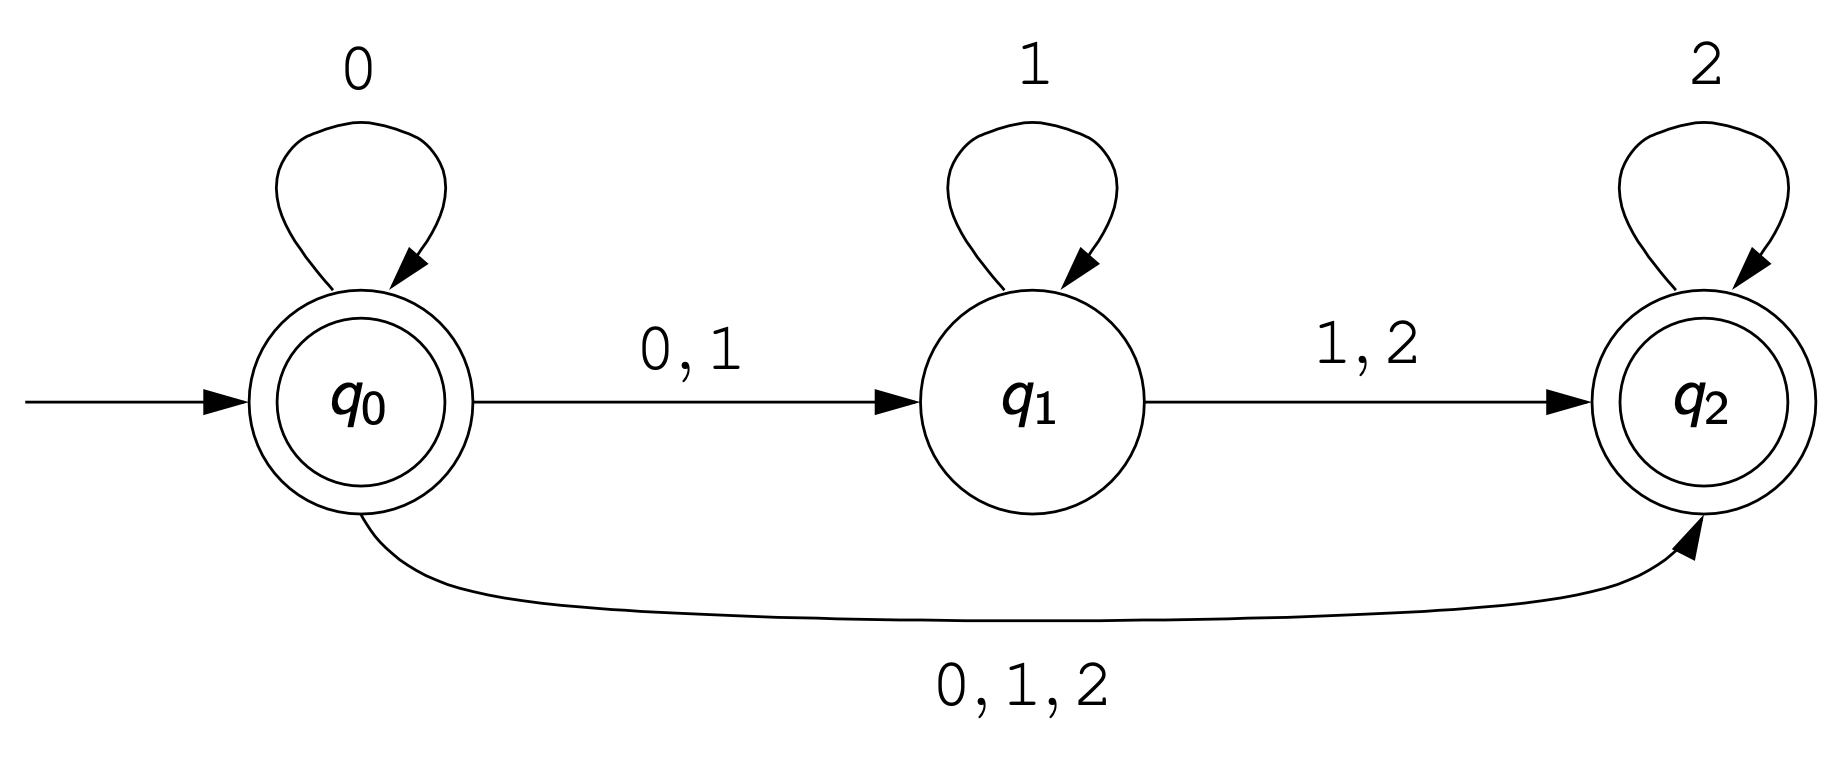
\includegraphics[width=0.95\columnwidth]{assets/epsilon2.png}

\subsection{Minimal DFA}
\definition{Minimal DFA}{A DFA $M'$ is minimal iif for any other DFA $M$ that recognizes the same language $|Q'|\le|Q|$}
\paragraph{Algorithm to minimize a DFA}
Idea: determine all the classes of states that are equivalent, and use these equivalence classes as the states of the minimal automaton. Two states are equivalent if and only if from both states any word leads or does not lead to a final state.

\begin{enumerate}
  \item Remove all stats of $M$ that are useless. A state $q$ is useless iif there is no word $w$ such that $\delta^*(q_0,w)=q$ (unreachable state) or if there is no word $w$ such that $\delta^*(q,w)\in F$ (dead-end)
  \item Find all the equivalence classes of states according to the following relation $R$: the relation $R(q,q')$ is true iif for any word $w\in\Sigma'^*$
        \begin{itemize}
          \item either $\delta^*(q,w)\in F$ and $\delta^*(q',w)\in F$
          \item or $\delta^*(q,w)\notin F$ and $\delta^*(q',w)\notin F$
        \end{itemize}
        It is sufficient to consider the words $w$ with $|w|\leq |Q|$
  \item The minimal automaton is $M^{\prime}=\langle Q^{\prime}, \Sigma, \delta^{\prime}, q_0^{\prime}, F^{\prime}\rangle$ where
        \begin{itemize}
          \item $Q^{\prime}=\{[q]\}$
          \item $q_0^{\prime}=[q_0]$
          \item $\delta^{\prime}([q], a)=[\delta(q, a)]$
          \item $F^{\prime}=\{[q] \mid q \in F\}$
        \end{itemize}
\end{enumerate}

\subsection{Regular Languages}
\definition{Regular Language}{A language recognized by a FSA recognizer.}
\begin{itemize}
  \item The \textbf{union of two regular languages} $L_1$ and $L_2$ $L_1\cup L_2$ is a regular language. Construct a $\epsilon$-NFA from $\text{FSA}_{L_1}$ and $\text{FSA}_{L_1}$ by introducing a new $q_0$ with $\epsilon$-transitions to $q_0$ of the FSAs and $\epsilon$-transitions from all accepting states from the FSAs to a new accepting global state.
  \item The \textbf{concatenation of two regular languages} $L_1$ and $L_2$ is still regular. $\epsilon$-transitions from a new $q_0$ to the initial state of $L_1$, then from all accepting of $L_1$ to the initial of $L_2$, then from all accepting of $L_2$ to a new global accepting.
  \item The \textbf{complement of a regular language} $L (\overline{L}=\Sigma^*\backslash L)$ is regular. Make every accepting state non-accepting and every non-accepting state accepting.
  \item The \textbf{iterative closure} $L^*$ is regular.
\end{itemize}

\subsection{Grammar}
Automatons recognize a language by consuming words, grammars generate words. Grammars are also called rewriting systems and rules rewriting rules or productions.

\begin{itemize}
  \item A \textbf{rule} is composed of a left-hand side $\alpha$ and a right-hand side $\beta$ surrounding an arrow: $\alpha\rightarrow\beta$
  \item Symbols are either \textbf{terminals} (symbols that compose the words generated by the grammar, denoted lowercase) or \textbf{nonterminals} (symbols mainly used in the rewriting process, denoted uppercase)
  \item A \textbf{term} is a sequence of term. and nonterm. symbols
  \item \textbf{rewriting} a term consists of applying a rule, thus replacing the l.h.s of the term with the r.h.s of the rule.
  \item Starting the rewriting process from a special rule called \textbf{axiom} and applying repetitively the rules, we obtain (not always) a term composed of terminal only. This is a word \textbf{generated} by the grammar.
  \item The set of words generated by the rewriting process is called the language \textbf{generated} by the grammar.
  \item The rewriting process is potentially nondeterministic, because any rules can be selected.
\end{itemize}

\definition{Grammar}{
  A grammar is a 4-tuple $G=\langle V_T, V_N, P, S\rangle$ where
  \begin{itemize}
    \item $V_T$ is a set of terminal symbols,
    \item $V_N$ is a set of nonterminal symbols such that $V_T \cap V_N=\varnothing$,
    \item $P$ is a set of rules $\alpha \rightarrow \beta$ where $\alpha$ and $\beta$ are sequences of terminals or nonterminals, but $\alpha$ must contain at least one nonterminal,
    \item $S \in V_N$ is the axiom or the initial symbol.
  \end{itemize}
}
Applying a single rule is called a \textbf{one-step derivation}, denoted by $\alpha\Rightarrow_G\beta$. A \textbf{derivation} is a sequence of one-step derivations, denoted by $\alpha\Rightarrow_G^*\beta$.\\

The language $L(G)$ \textbf{generated} by a grammar is the set of all the words which can be obtained or derived by rewriting from the axiom and do not contain any nonterminals.

\subsubsection{Regular Grammar}

\definition{Regular Grammars}{
  A grammar is right/left regular if for all rewriting rules $\alpha\rightarrow\beta$:
  \begin{enumerate}
    \item $|\alpha|=1$
    \item $\beta=a$, $\beta=\epsilon$, or
          \begin{itemize}
            \item $\beta=aB$ for right regular languages
            \item $\beta=Ba$ for left regular languages
          \end{itemize}
  \end{enumerate}
}
A language $L$ is recognized by a FSA iif $L$ is generated by a regular grammar.

\subsection{Regular Expressions}
\definition{Regular Expression (RE)}{Over an alphabet $\Sigma$:
  \begin{enumerate}
    \item $\varnothing$ is a RE that denotes the empty set,
    \item $\epsilon$ is a RE that denotes the set $\{\epsilon\}$
    \item for any $a \in \Sigma, a$ is a RE that denotes the set $\{a\}$
    \item if $r$ and $s$ are two REs which denotes the sets $R$ and $S$, respectively, then $(r+s),(r s)$ and $\left(r^*\right)$ are REs that denote the sets $R \cup S, R \cdot S$, and $R^*$, respectively.
  \end{enumerate}
}

\definition{Pumping Lemma}{
  The pumping lemma, states that if a language is regular, then it is possible to identify, for every word $w$ of the language, at least one way to split $w$ as $w = xyz$. If the word $y$ is pumped ($w^i$ for any $i \ge 0$), then $xy^iz$ belongs to the language as well.
}
Let $L$ be an infinite regular language. Then, there exists a constant $n$ such that, for any word $w$ of $L$, where $|w|\ge n$, we can write $w=xyz$ with $|xy|\le n$, $|y|\ge 1$ and for all $i\ge 0$, $xy^iz$ belongs to $L$. $n\le |Q|$ where $|Q|$ is the number of states of the minimal automaton that accepts $L$.

tl;dr: $w$ is a word accepted by a minimal FSA with $n$ states, but $|w| > n$. Thus, a certain path through the FSA is repeated. Any word where this path is repeated an arbitrary amount of times is also accepted by the FSA and thus belongs to the language.

Used to proof a language is not regular. To do this, split a word at each possible place, show how a changed $i$ is not in the language anymore.

\section{Pushdown Automata and Context Free Languages}

\subsection{Pushdown Automaton (PDA)}

\definition{Pushdown Automaton}{
  A 6-tuple $M=\left\langle Q, \Sigma, \Gamma, \delta, q_0, \triangleleft\right\rangle$ where
  \begin{itemize}
    \item $Q$ is a finite set of states
    \item $\Sigma$ is an input alphabet
    \item $\Gamma$ is an auxiliary alphabet (symbols of the stack) such that $\Gamma \cap \Sigma=\varnothing$
    \item $\delta: Q \times(\Sigma \cup\{\epsilon\}) \times \Gamma \rightarrow Q \times \Gamma^*$ is a transition function
    \item $q_0 \in Q$ is the initial state
    \item $\triangleleft \in \Gamma$ is a special symbol which indicates that the stack is empty
  \end{itemize}
  PDA recognizers further add a set of final states $F$.
}
Convention (in graphs): $(a,Z|\alpha)$ is a transition where $a$ is the input symbol, $Z$ is the symbol at the top of the stack before applying the transition function, and $\alpha$ is the content of the stack after.

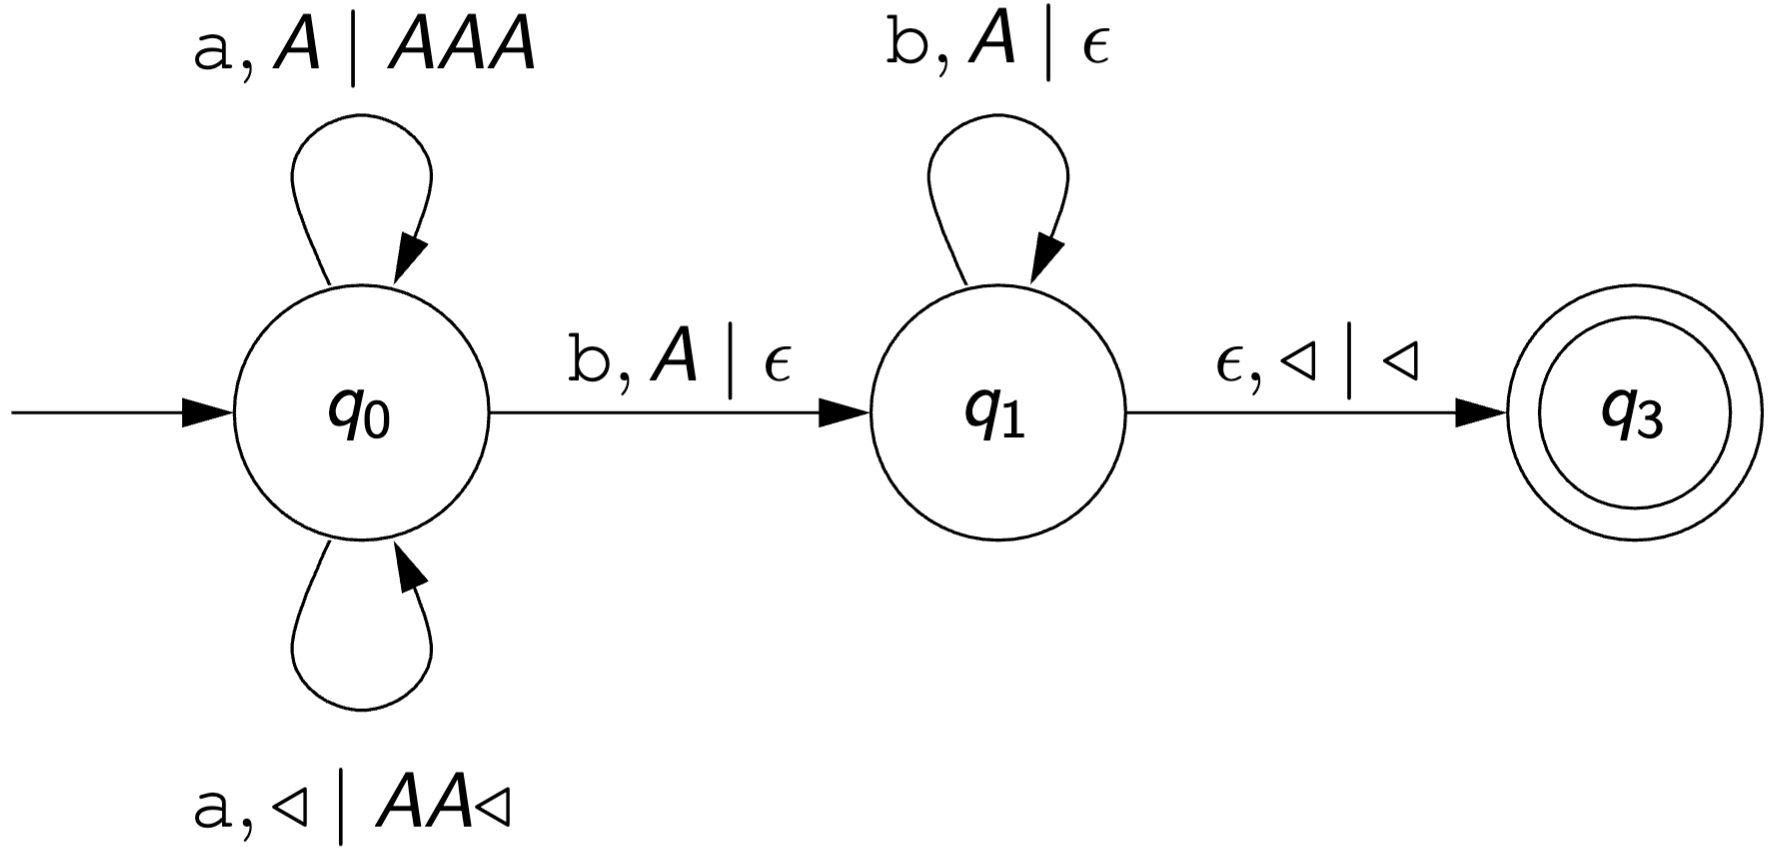
\includegraphics[width=0.95\columnwidth]{assets/pda.png}

\definition{Nondeterministic PDAs}{
  A PDA with $\delta: Q \times(\Sigma \cup\{\epsilon\}) \times \Gamma \rightarrow \mathcal{P}(Q\times \Gamma^*)$.
}
The classes of languages recognized by DPDAs and NPDAs are \textit{not the same}. There exists a context-free language which is not recognized by any DPDA.

Example: $L=\{a^nb^n|n\ge1\}\cup\{a^nb^2n|n\ge1\}$, where there are two transitions to the second part of the automaton, one for the right, one for the left version.

\subsection{Context-Free Grammars}
\definition{Context-Free Grammar}{
  A context-free grammar $G=\langle V_T,V_N,P,S\rangle$ is a grammar whose productions $\alpha\rightarrow\beta$:
  \begin{enumerate}
    \item $|\alpha|=1$ and $\alpha\in V_N$
    \item $\beta$ is a sequence of terminals and/or nonterminals
  \end{enumerate}
}
The language generated by a context-free grammar $G$ is called a context-free language, we denote this language $L(G)$.

\definition{Backus-Naur Form (BNF)}{
  A notation of context-free grammars:
  \begin{itemize}
    \item Nonterminals are strings
    \item Terminals are (single or double) quoted strings or symbols
    \item $=$ corresponds to the arrow of a production
    \item $|$ corresponds to alternative
    \item $,$ concatenates elements
    \item $;$ terminates a production
  \end{itemize}
}

\definition{Extended BNF (EBNF)}{
  Superset of BNF:
  \begin{itemize}
    \item Parentheses can be use to group elements
    \item $[\gamma]$ means $\gamma$ is optional (appear $0$ or $1$ times)
    \item $\{\gamma\}$ means $\gamma$ can be repeated $0$ or more times
  \end{itemize}
}

\definition{Ambiguous Grammar and Language}{
  A grammar $G$ is ambiguous iif there exists a word $w\in L(G)$ such that $w$ has more than one parse tree ($\stackrel{?}{=}$ derivation).

  A language $L$ is ambiguous iif all grammars that generate $L$ are ambiguous.
}

A language $L$ is recognized by a nondeterministic PDA iif $L$ is a context-free language.

\paragraph{Pumping Lemma for Context-Free Languages}
If $L$ is a context-free language, then there exists a constant $n$ such that for any word $w$ of $L$, with $|w|\le n$, we can split the word $w=uvxyz$ with
\begin{enumerate}
  \item $|vy|\ge 1$
  \item $|vxy|\le n$
  \item $\forall i\ge 0, uv^ixy^iz\in L$
\end{enumerate}
This is used to proof that a language is not context free.

\section{Lexical Analysis and Parsing}

\definition{Parsing}{
  Processing an input text consists generally in, verifying that the structure of the text is correct, and in performing some operations using the text under analysis.

  In general, a grammar describes the syntactical structure of the input text. Thus, verifying that the structure of the text is correct consists in making sure that the text is in conformity with the grammar. This is parsing.
}

\subsection{Lexical Analysis}

\definition{Lexical Analysis}{
  The lexical analysis activity consists in reading a text character by character and in grouping the characters that form terminals of the grammar. Such terminals are usually called \textbf{tokens}.
}
A \textbf{lexer} or \textbf{scanner} is a program that performs the lexical analysis of an input text.

Terminals can generally be described by regular expressions, therefore lexers are usually implemented based on RE and/or FSAs and then transformed to minimized DFAs.

\subsection{Syntax Analysis}
\definition{Syntax Analysis}{
  Syntax analysis is veryifing that the input text is well structured, i.e. the input is in cinformity with a given grammar.
}

For the verification of the conformity with respect of a given grammar, we build the parse tree of the input text. An input text is syntactically correct iif the parse tree can be built.

A program that performs this activity is called a parser. The main task of a parser is to create the parse tree of its input using a grammar that describes the structure of its input. Note that a parser uses a lexer for the lexical analysis.

For context-free languages, this can be done easily, and since programming languages generally are context-free and unambiguous, this can be done, but certain aspects of programming languages cannot be expressed by context-free grammars, such as declare-before-use rules or type checking.

\definition{Parse Tree}{A parse tree illustrates graphically how a given word is generated by a grammar, i.e. which productions are used to generate a given word.}

Bottom-up analysis: "Use grammar backwards", start at the bottom of the parse tree and thus with terminals, combine them into nonterminals until you find the initial symbol.

Top-down analysis: Apply derivations successively from the first rewriting rule. This is easier but has some limitations.

\subsubsection{Recursive Descent}

\definition{Recursive Descent}{Recursive Descent is a top-down approach in which we execute a program that applies a set of recursive functions (or methods) to process the input.}

\definition{LL(1) Grammars}{
  The class of LL(1) grammars is a sub-set of context-free grammars. One way of parsing such grammars is to use recursive descent parsers in which no backtracking is required. \textbf{L}eft to right \textbf{L}eft-most derivation with \textbf{1} token lookahead.
}

Left-most derivation: left-most rule is expanded first. (=Depth-First Search)
\definition{Left Recursion}{
  A rule of a context-free grammar has \textbf{immediate left recursion} if it has the form $X\rightarrow X\alpha|\beta$ (or multiple $X\alpha_i$s or $\beta_i$s).
  \textbf{General left recursion} can occur through several rules, e.g. (this is both)
  $$\begin{aligned}
      S & \rightarrow Aa|b           \\
      A & \rightarrow Ac|Sd|\epsilon
    \end{aligned}$$
}

\paragraph{Left Recursion Removal for Immediate LR}
$$
  \begin{aligned}
    X              & \rightarrow X\alpha_1|X\alpha_2|\ldots|X\alpha_n|\beta_1|\beta_2|\ldots|\beta_m \\
    \text{becomes} &                                                                                 \\
    X              & \rightarrow \beta_1X'|\beta_2X'|\ldots|\beta_mX'                                \\
    X'             & \rightarrow \alpha_1X'|\alpha_2X'|\ldots|\alpha_nX'|\epsilon
  \end{aligned}
$$


\paragraph{Left-Factoring}
$$
  \begin{aligned}
    X  & \rightarrow \alpha\beta|\alpha\gamma \\
    \text{becomes}                            \\
    X  & \rightarrow \alpha X'                \\
    X' & \rightarrow \beta|\gamma
  \end{aligned}
$$

\definition{LL(k) Grammars}{A grammar is LL(k) iif there exists a recursive descent parser that uses $k$ tokens lookahead.}
The class of LL(k) grammars strictly includes the class of LL(k-1) grammars. Most LL(k) grammars can be translated to LL(1), but not all.

\definition{LR(k) Grammars}{LR(k) grammars can be analyzed with parsers based on the bottom-up technique with k token lookahead.}
\textbf{L}eft to right \textbf{R}ight-most derivation with $k$ tokens lookahead. Any LR(k) grammar can be translated into a LR(1) grammar. If actions can be arbitrarily inserted into production rules, then LR(k) class strictly includes LR(k-1).

\paragraph{Comparing LL and LR parsers}
LR parsers are much more complex, more difficult to use, less efficient, require more memory, only used through parser generators. Due to the size of tables of LR parsers, parser generators work only for a sub-class of LR grammars called LALR(1) (Lookahead LR). For LR parsers left-recursion is allowed, more complex context-free languages can be analyzed, errors are detected as soon as they are encountered, almost all programming languages can be parsed by bottom-up parsers.

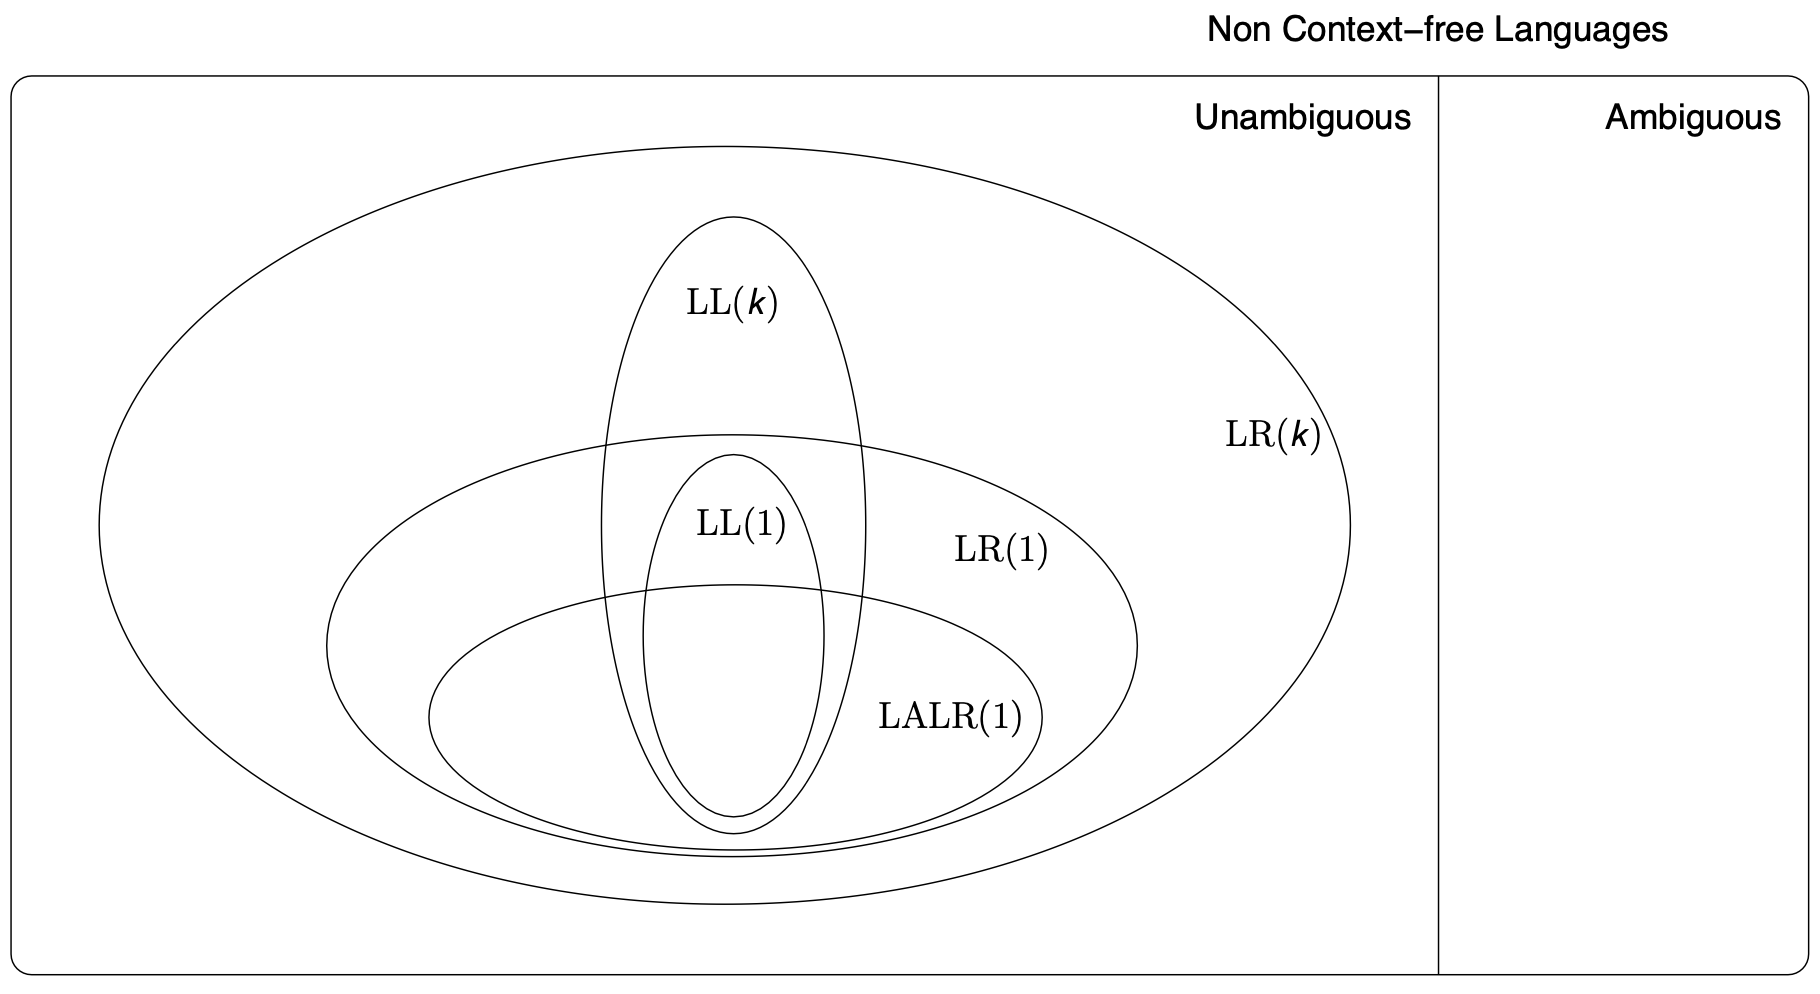
\includegraphics[width=0.95\columnwidth]{assets/parsers.png}

\section{Turing Machines (TM)}

\definition{Deterministic $k$-tapes Turing Machine}{
  A deterministic $k$-tapes TM with $k \geq 0$ (auxiliary tapes) is a 8-tuple $M=\langle Q, \Sigma, \Gamma, O, \delta, q_0, \square, F\rangle$ where
  \begin{itemize}
    \item $Q$ is a finite set of states,
    \item $\Sigma$ is an input alphabet,
    \item $\Gamma$ is an auxiliary alphabet (for auxiliary tapes),
    \item $O$ is an output alphabet,
    \item $F \subseteq Q$ is a set of final states,
    \item $q_0$ an initial state,
    \item $\square$ is the blank symbol,
    \item $\delta: Q \times \Sigma \times \Gamma^k \rightarrow Q \times \Gamma^k \times O \times\{R, S\} \times\{R, L, S\}^k \times\{R, S\}$ is a transition function with \textbf{R}ight, \textbf{L}eft, or \textbf{S}tationary
  \end{itemize}
}

A language recognized by a Turing Machine is called a \textbf{recursively enumerable language}.

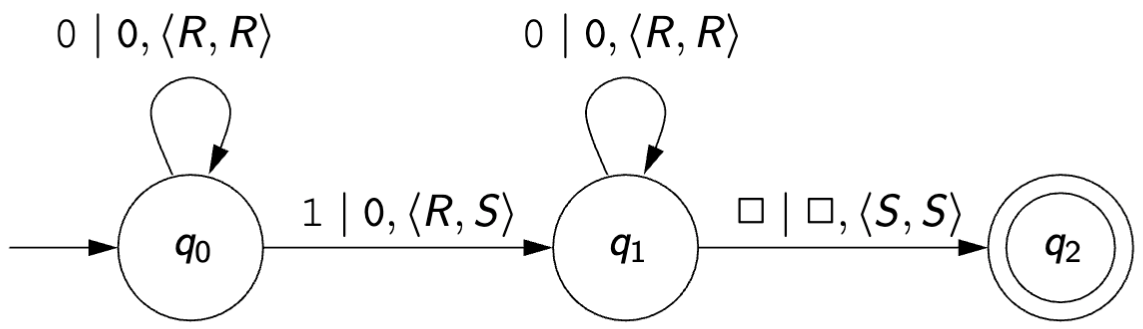
\includegraphics[width=0.95\columnwidth]{assets/tm.png}

Transitions are marked as follows: $$i,\quad r_1, \ldots, r_k \quad|\quad r'_1,\ldots,r'_k,\quad o,\quad \langle M_0,\ldots, M_{k+1}\rangle$$ with the input tape symbol $i$, aux tape symbols $r_1,\ldots,r_k$, new aux tape symbols $r'_1,\ldots,r'_k$, output tape symbol $o$ and movements $M_0$ (input tape), $M_1,\ldots M_k$ (aux tapes) and $M_{k+1}$ (output tape). Input and output tapes cannot move to the left.

\definition{Single Tape TM}{
  A single tape TM $M$ is a 7-tuple $M=\langle Q, \Sigma, \Gamma, \delta, q_0, \square, F\rangle$ where
  \begin{itemize}
    \item $Q$ is a finite set of states,
    \item $\Gamma$ is the finite set of symbols of the tape,
    \item $\Sigma$ is the input alphabet with $\Sigma=\Gamma\backslash\square$,
    \item $\delta: Q \times \Sigma \rightarrow Q \times \Gamma \times\{L,R\}$ is a transition function with \textbf{R}ight or \textbf{L}eft
    \item $q_0$ an initial state,
    \item $\square$ is the initial blank symbol,
    \item $F \subseteq Q$ is a set of final states,
  \end{itemize}
}

\definition{Nondeterministic $k$-tapes TM}{
A nondeterministic $k$-tapes Turing machine is a 8-tuple $M=\langle Q, \Sigma, \Gamma, O, \delta, q_0, \square, F\rangle$ where only the transition function
$$
  \delta: Q \times \Sigma \times \Gamma^k \rightarrow \mathcal{P}(Q) \times \Gamma^k \times\{R, L, S\}^{k+1}
$$
is different from the deterministic model. The power set is used to model nondeterminism, as for nondeterministic FSA.
}

Single tape nondeterministic TMs recognize a language iif a deterministic TM recognizes it.

\definition{Grammar Without Restrictions}{A grammar without restrictions is a grammar $G=\langle V_T, V_N, P,S\rangle$ where the rules looke like $\alpha\rightarrow\beta$ with $\alpha\neq\epsilon$ and $\alpha$, $\beta$ are sequences of terminals and nonterminals.}

A language $L$ is generated by a grammar without restrictions iff a TM recognizes $L$.

\definition{Context Sensitive Languages and Grammars}{
  A context sensitive language is generated by a context sensitive grammar, i.e. a grammar that has rewriting rules $\alpha\rightarrow\beta$ with $|\alpha|\le|\beta|$.
}

Context-sensitive grammars correspond to linear bounded automata (LBA).

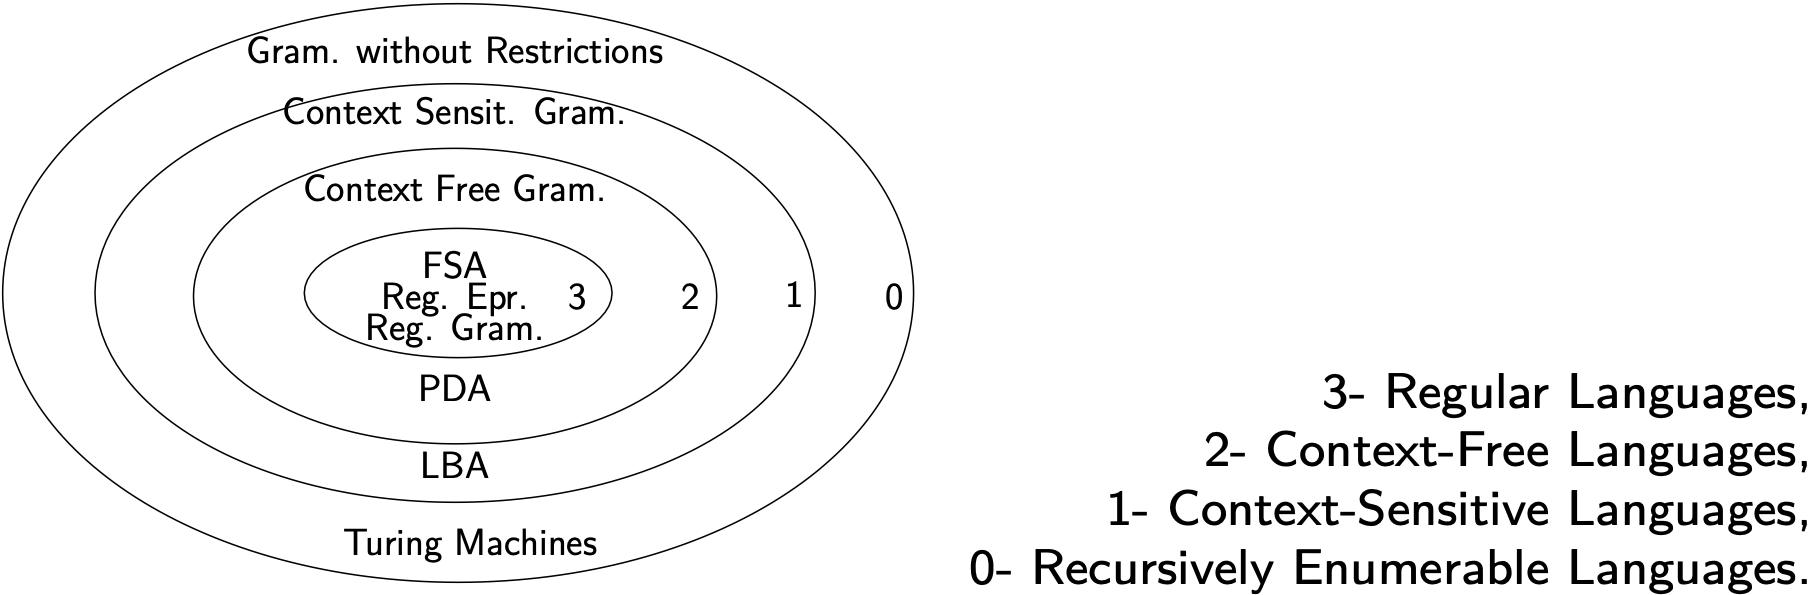
\includegraphics[width=0.95\columnwidth]{assets/languages.png}

\section{Decidability and Reducibility}
\definition{Algorithm}{
  A Finite collection of basic instructions or operations that perform some tasks. An algorithm always stops.

  Church-Turing thesis: TM algorithms equal intuitive notion of algorithms.
}

A language is called \textbf{Turing-recognizable}, if a TM accepts all words that belong to it, as opposed to rejecting it or looping infinitely. It is called \textbf{Turing-decidable}, if the machine stops for all inputs.

\subsection{Decidability}

\subsubsection{Decidable problems}
\begin{itemize}
  \item Acceptance problem for DFAs $A_{\text{DFA}}$ is decidable (Whether a DFA $B$ accepts a given string $w$, or testing whether $\langle B,w\rangle$ is a member of $A_\text{DFA}$), by building a TM that simulates the DFA.
  \item Acceptance problem for NFAs $A_\text{NFA}$ is decidable by building a TM that turns the NFA into a DFA and simulates it.
  \item Testing if a DFA accepts only the empty language ($E_\text{DFA}$) is decidable given an algorithm that tests if there is a path between any two nodes of a graph.
  \item $EQ_\text{DFA}$ is decidable by designing a DFA such that $L(C)=(L(A)\cap\overline{L(B)})\cup(\overline{L(A)}\cap L(B))$ with $L(C)=\varnothing$ iif $L(A)=L(B)$.
  \item $A_\text{CFG}$ is decidable by designing a TM that converts the context-free grammar into Chomsky normal form, listing all derivations with $2n-1$ steps where $n=|w|$ (except $n=0$, then list all derivations with $1$ step), and accepting if any of these derivations generate $w$.
  \item Every context-free language is decidable. Turning a PDA/CFG into a TM does not generally work because of possible infinite loops (non-deterministic PDAs $\not\equiv$ deterministic PDAs). Just use the above though.
\end{itemize}

\definition{Universal Turing Machine}{A TM that can simulate any other TM from a description.}


\subsubsection{Undecidable problems}
\begin{itemize}
  \item $A_\text{TM}=\{\langle M,w\rangle | M\text{ is a TM and } M \text{ accepts }w\}$ is undecidable. It is Turing-recognizable by constructing a universal TM that simulates $M$, but will loop if $M$ loops. Halting problem: suppose that $H(\langle M,w\rangle)$ is a decider for $A_\text{TM}$, now build $D(\langle M\rangle)=!H(\langle M, \langle M\rangle\rangle)$. Now, run $D(\langle D\rangle)$. It accepts if $D$ does not accept $\langle D\rangle$ and rejects if $D$ accepts $\langle D\rangle$. Neither $D$ nor $H$ can exist.
  \item $HALT_\text{TM}$ is undecidable, because if there was such a TM, it could be used to calculate $A_\text{TM}$, by checking if it halts, returning false otherwise and if true, simulating the TM.
  \item $E_\text{TM}$ is undecidable, because one can construct a wrapper for the TM under test $M$, that rejects any input $x$ if it isn't equal to $w$ and otherwise runs $M$. Assuming there is a TM that solves $E_\text{TM}$, run it on the wrapper and invert the result. This is equal to $A_\text{TM}$.
  \item $EQ_\text{TM}$ is undecidable because if one of the TMs passed is a TM that only accepts the empty language, this would solve $E_\text{TM}$.
\end{itemize}

\paragraph{Diagonalization}
Imagine a table with rows of all possible TMs, columns of all possible inputs, and field with the evaluation of the TM on the input. $D$ is a valid TM and a valid input and thus a row and a column. The row with $D$ is the opposite as the values on the diagonal. There's an obvious contradiction when $D$ comes to $\langle D\rangle$, because it needs to be the opposite of itself.

\subsubsection{Problems that are not Turing-recognizable}
Basics:
\begin{itemize}
  \item If a language $A$ is decidable by a decider $M$, its complement is also decidable (invert the answer of $M$).
  \item A language is decidable iif it is Turing-recognizable and its complement is also Turing-recognizable.
        \begin{itemize}
          \item The complement of a decidable language is decidable and every decidable language is Turing-recognizable.
          \item Let $M_1$ and $M_2$ be two recognizers for languages $A$ and $\overline{A}$. Run both on an input, at least one needs to halt (since recognizers halt on inputs that belong to the language), use that information to decide.
        \end{itemize}
\end{itemize}

Examples:
\begin{itemize}
  \item $\overline{A_\text{TM}}$ is not Turing-recognizable, since $A_\text{TM}$ is Turing-recognizable, but not decidable. So if $\overline{A_\text{TM}}$ were Turing-recognizable, it would also need to be decidable (see Basics).
  \item $\overline{EQ_\text{TM}}$ is not Turing-recognizable, because there is a reduction from $A_\text{TM}$ to $EQ_\text{TM}$.
\end{itemize}

\subsection{Reducibility}
\definition{Computable Function}{A function $f:\Sigma^*\rightarrow\Sigma^*$, if some TM $M$ halts on every input $w$ and writes $f(w)$ on its tape.}
\definition{Mapping reducible}{A language $A$ is mapping reducible to a language $B$, written $A\le_m B$, if there is a computable function $f$ such that for every $w$, $w\in A\Longleftrightarrow f(w)\in B$.}
$f$ is called the \textbf{reduction} of $A$ to $B$.

\begin{center}
  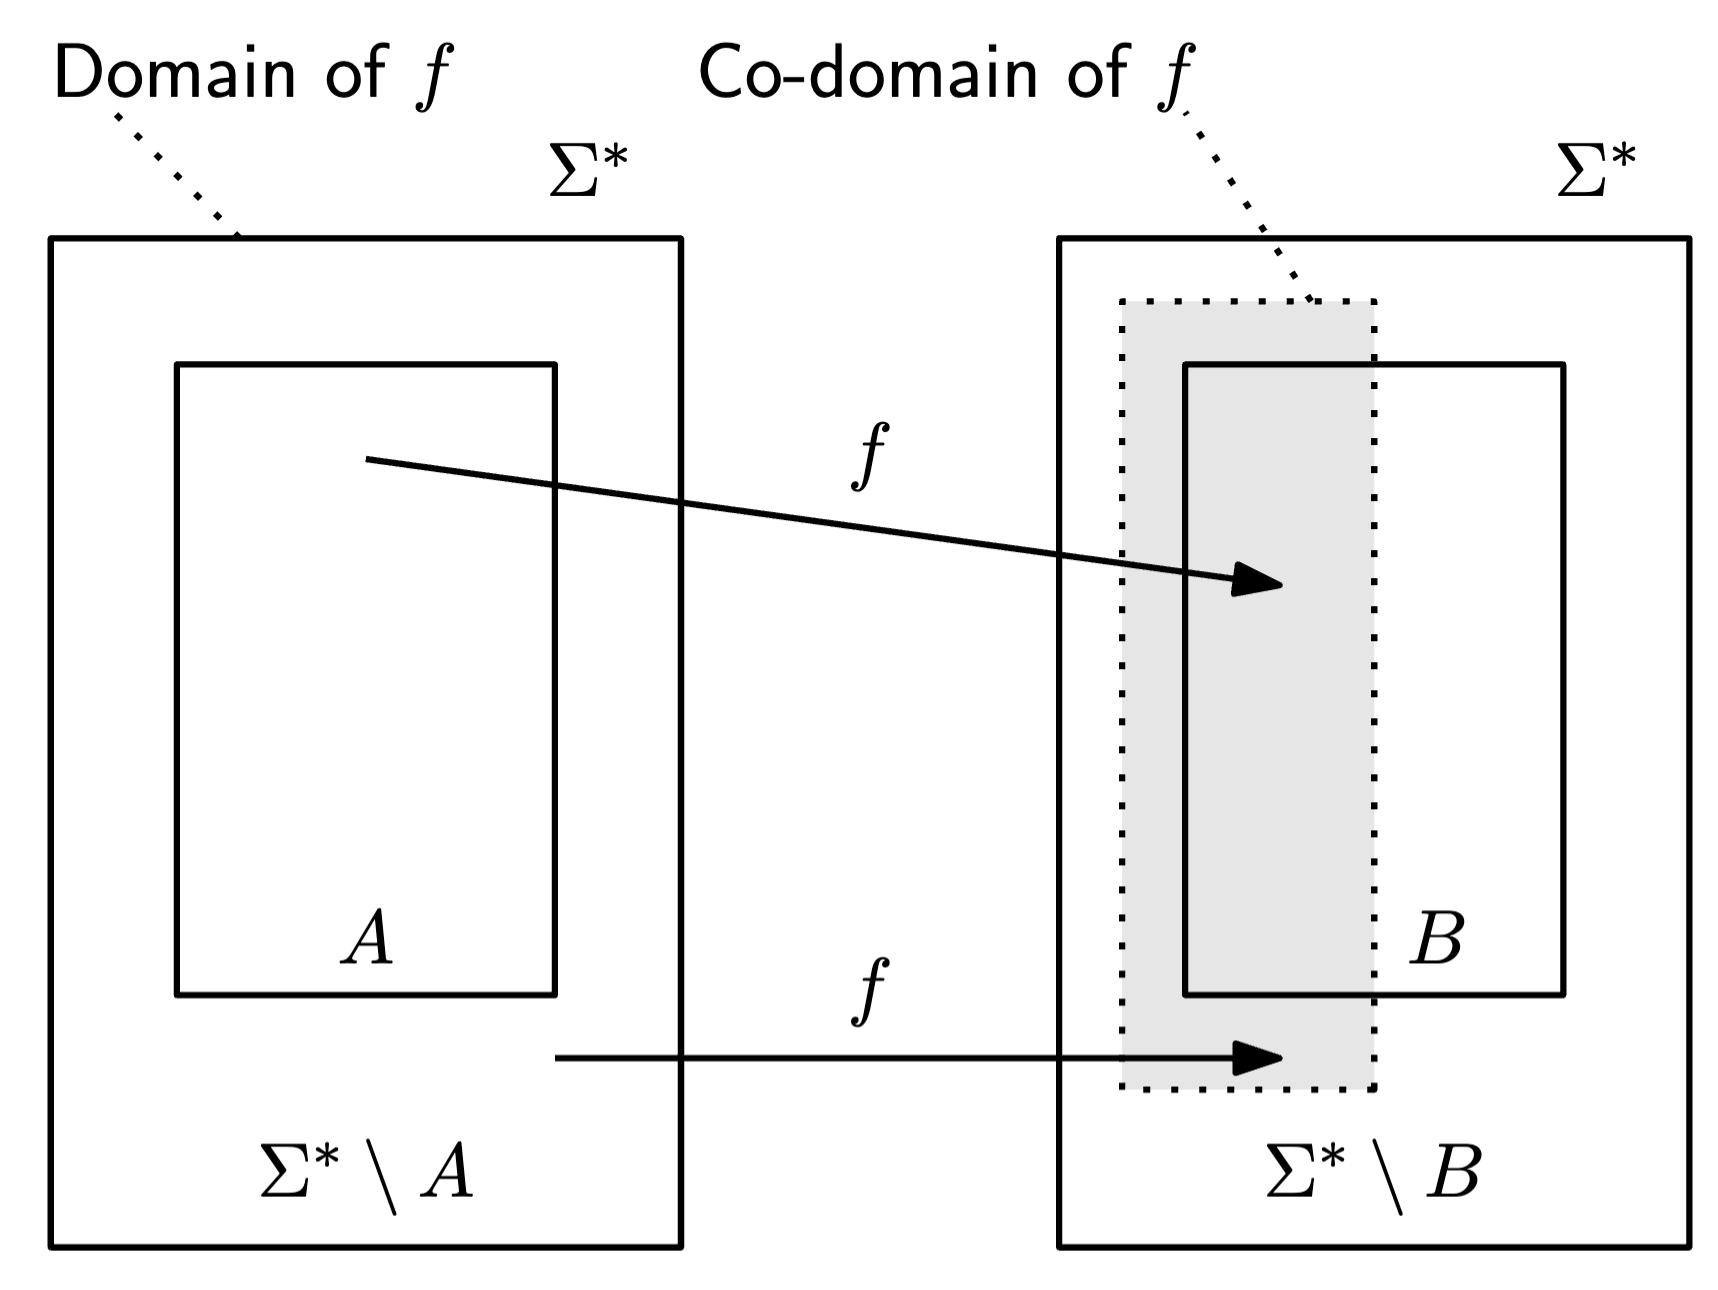
\includegraphics[width=0.80\columnwidth]{assets/f.png}
  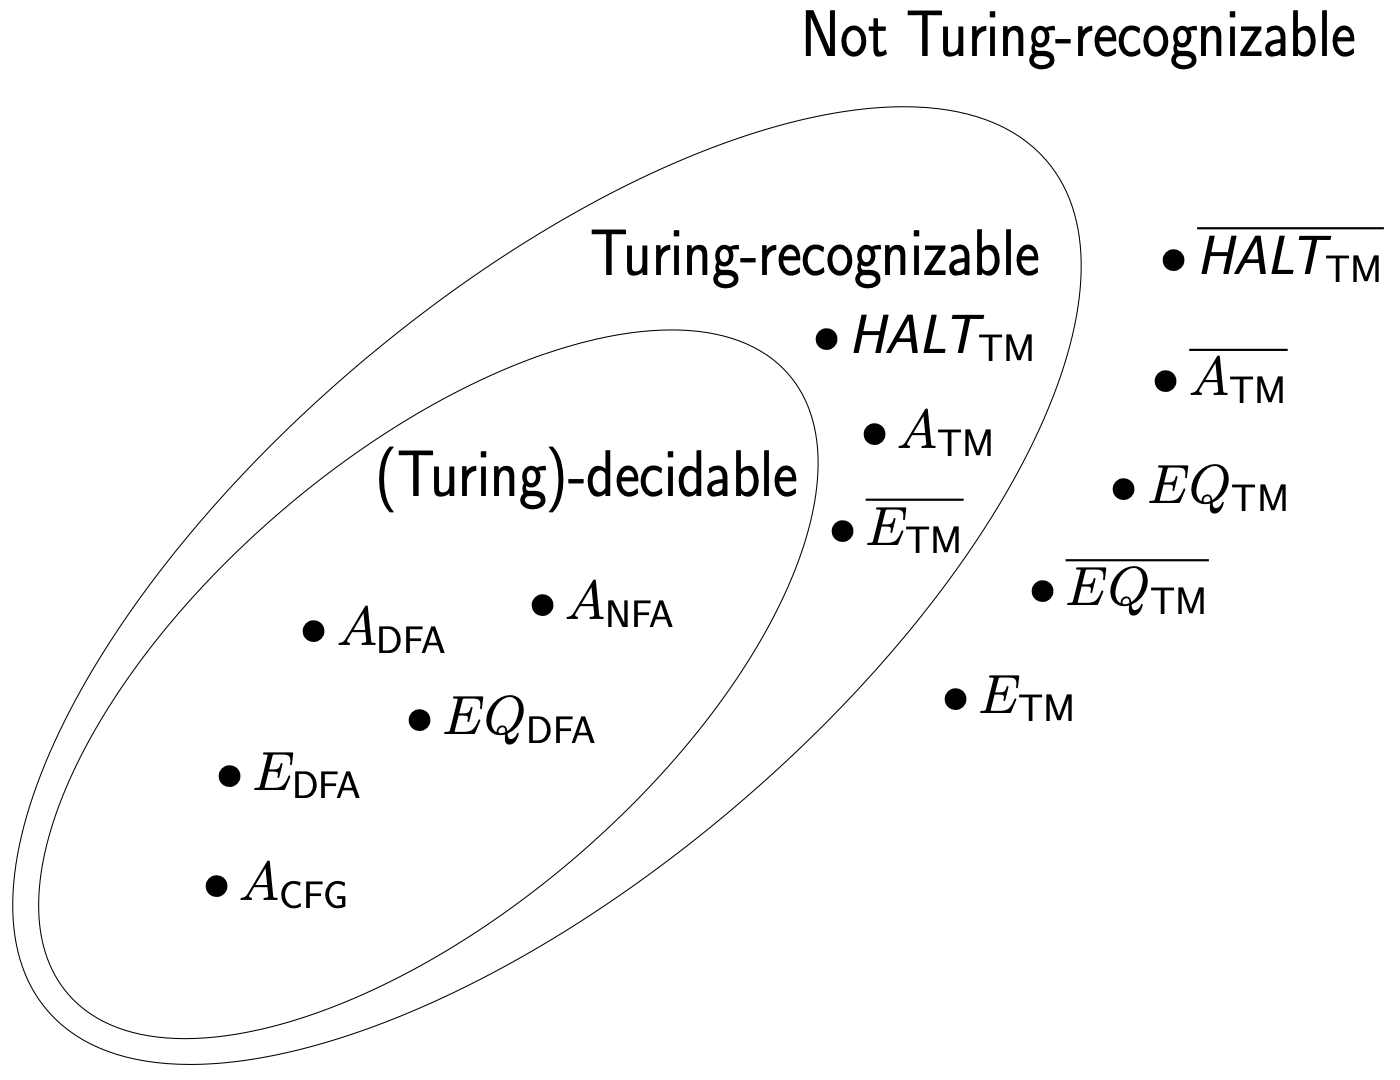
\includegraphics[width=0.95\columnwidth]{assets/turing-classes.png}
\end{center}

\subsubsection{Theorems}
Meta:
\begin{itemize}
  \item If $A\le_m B$ and $B$ is solvable, then $A$ is solvable.
  \item If $A\le_m B$ and $A$ is unsolvable, then $B$ is unsolvable.
  \item $A\le_m B$ says that a computer can transform any instance of $A$ into an instance of $B$ such that the answer to $B$ is the answer to $A$.
\end{itemize}
Actual:
\begin{itemize}
  \item If $A\le_m B$ and $B$ is decidable, then $A$ is decidable, because we can apply $f$ to $w$ on a TM and use that result to decide $w$ on $A$.
  \item If $A\le_m B$ and $B$ is Turing-recognizable, then $A$ is Turing-recognizable, same argument.
  \item If $A\le_m B$ and $A$ is undecidable, then $B$ is undecidable.
        \begin{itemize}
          \item Assume $B$ is decidable, construct a TM that uses $B$ to decide A, therefore contradiction.
          \item Problem $A$ reduces to problem $B$ iff a solver for $B$ can be used to solve problem $A$.
          \item tl;dr: Construct a machine using a solver to $B$ that solves the halting problem, $\text{HALT}_\text{TM}\le_m  B$ notated, where $B$ is your problem. Alternatively, reduce to $\overline{B}$, since if $\overline{B}$ is decidable, $B$ is also decidable.
        \end{itemize}
  \item If $A\le_m B$ and $A$ is not Turing-recognizable, then $B$ is not Turing-recognizable.
  \item $A\le_m B \Longleftrightarrow \overline{A}\le_m \overline{B}$
  \item To prove that $B$ is not Turing-recognizable, we may show that $A_\text{TM}\le_m \overline{B}$. If this holds, and $B$ were also Turing-recognizable, then $A$ would be Turing-recognizable (rule 2 here), thus $A$ and $\overline{A}$ would be Turing-recognizable, thus $A$ would be decidable, which it obviously isn't.
\end{itemize}

\section{Complexity, NP, NP-Completeness}

\definition{Running Time or Time Complexity}{The running time or time complexity of a deterministic TM $M$ that always halts is the function $F:\mathbb{N}\rightarrow\mathbb{N}$, where $f(n)$ is the number of steps used by $M$ on any input of length $n$.}

If $f(n)$ is the running time of $M$, we say that $M$ runs in time $f(n)$ and that $M$ is an $f(n)$ time TM.

\definition{Big-O Notation}{Let $f$ and $g$ be the functions $f,g:\mathbb{N}->\mathbb{R}^+$. We say that $f(n)=O(g(n))$ if $c,n_0\in\mathbb{N}$ exist such that for every $n\ge n_0$ $f(n)\le cg(n)$.}

$f(n)=O(g(n))$ means that $g(n)$ is an upper bound for $f(n)$, or more precisely, $g(n)$ is an asymptotic upper bound for $f(n)$.

Because changing the base of a $\log$ only adds a factor, we can ignore it.

\definition{Small-o Notation}{
  Let $f$ and $g$ be the functions $f,g:\mathbb{N}\rightarrow\mathbb{R}^+$. We say that $f(n)=o(g(n))$ if $\displaystyle\lim_{n\rightarrow\infty}\frac{f(n)}{g(n)}=0$.
}
In other words, $f(n)=o(g(n))$ means that for any real number $c>0$, there exists $n_0$ such that $f(n)<cg(n)$ for all $n\ge n_0$. Informally, $g(n)$ grows much faster than $f(n)$.

Examples:
\begin{itemize}
  \item $\sqrt{n}=o(n)$
  \item $n=o(n\log\log n)$
  \item $n\log\log n=o(n\log)$
  \item $n\log n =o(n^2)$
  \item $n^2=o(n^3)$
  \item $n^2\neq o(3n^2)$
\end{itemize}

\definition{Time Complexity Class}{Let $t:\mathbb{N}\rightarrow\mathbb{R}^+$ be a function. Define the time complexity class, $\text{TIME}(t(n))$ to be the collection of all languages that are decidable by a deterministic Turing machine in time $O(t(n))$.}

  \subsection{Time Complexities of TMs}
  \begin{itemize}
    \item Let $t(n)$ be a function, where $t(n)\ge n$. Then every $t(n)$ time multi tape TM has an equivalent $O(t^2(n))$ time single tape TM.
    \item Let $N$ be a nondeterministic TM decider. The running time of $N$ is the function $f:\mathbb{N}\rightarrow\mathbb{N}$, where $f(n)$ is the maximum number of steps that $N$ uses on any branch of its computation any input of length $n$.
    \item Let $t(n)$ be a function where $t(n)\ge n$. Then every $t(n)$ time nondeterministic single tape TM has an equivalent $2^{O(t(n))}$ time deterministic single tape TM.
  \end{itemize}

  \subsection{The Classes P and NP}
  There is at most a quadratic or \textbf{polynomial} difference between deterministic single and multi tape TMs, but an \textbf{exponential} differences between deterministic and nondeterministic TMs.
  \definition{The Class P}{P is the class of languages that are decidable in polynomial time with a deterministic single tape TM, or $\displaystyle \text{P}=\bigcup_k\text{TIME}(n^k)$.}
  Examples of languages in P:
  \begin{itemize}
    \item $\text{PATH}$: Does a directed graph have a directed path between two given nodes? (Proof: Starting with the start node, iteratively taint new reachable nodes until there are none (at most $m$ steps). Accept if the target is tainted.)
    \item $\text{RELPRIME}$: Are two natural numbers relatively prime?
    \item Every context-free language decision. (Thus parsing of programming languages!)
    \item $\text{COMPOSITE}$: $\{x|x=pq,\text{ for integers }p,q>1\}$
    \item $\text{2SAT}$! ($\text{2SAT}\le_P \text{3SAT}$, but $\text{3SAT}\not\le_P\text{2SAT}$)
  \end{itemize}

  \definition{Verifier}{A verifier for a language $A$ is an algorithm $V$, where $A=\{w|V\text{ accepts }\langle w,c\rangle\text{ for some string }c\}$.}
  The time of a verifier is only measured in terms of the length of $w$. A language is \textbf{polynomially verifiable} if it has a polynomial time verifier. $c$ is called the certificate of membership in $A$, e.g. the certificate for a string $\langle G,s,t\rangle\in\text{HAMPATH}$ is the path from $s$ to $t$, for $\text{COMPOSITE}$, it is one of the divisors of $x$.

  \definition{The class NP}{NP is the class of languages that have polynomial time verifiers. A language is in NP iif it is decided by a nondeterministic polynomial time TM.}
  A language may belong to NP only ($\text{HAMPATH}$), or to both NP and P ($\text{COMPOSITE}$). P is a subset of NP.

  \definition{NTIME}{$\text{NTIME}(t(n))$ is the nondeterministic time complexity class that contains all languages decided by a $O(t(n))$ time nondeterministic TM.}

$\displaystyle\text{NP}=\bigcup_k \text{NTIME}(n^k)$

Examples of languages in NP:
\begin{itemize}
  \item $\text{HAMPATH}$: What is the directed path through a directed graph that visits each node exactly once?
  \item $\text{CLIQUE}$: A $k-\text{clique}$ is a subgraph of a undirected graph wherein every two nodes are connected by an edge with $k$ nodes. Does a certain undirected graph contain a clique of size $k$? (Proof: Either build a verifier that tests whether enough nodes are in the subgraph and if all edges are there, or build a nondeterministic TM that (nondeterministically) selects a subset of nodes and checks if all edges are present).
  \item $\text{SUBSET-SUM}$: Does a subcollection (repetition allowed!) of a collection of integers $x_1,\ldots,x_k$ sum up to a target number $t$? (Proof: Verifier that tests whether all given elements belong to the collection, and if the sum matches)
\end{itemize}

\definition{The Class \NoCaseChange{co-NP}}{Languages for which the complement is in NP.}

$\overline{\text{HAMPATH}}$, $\overline{\text{CLIQUE}}$, and $\overline{\text{SUBSET-SUM}}$ are not obviously in NP. Probably NP$\neq$co-NP, but certainly P=co-P.

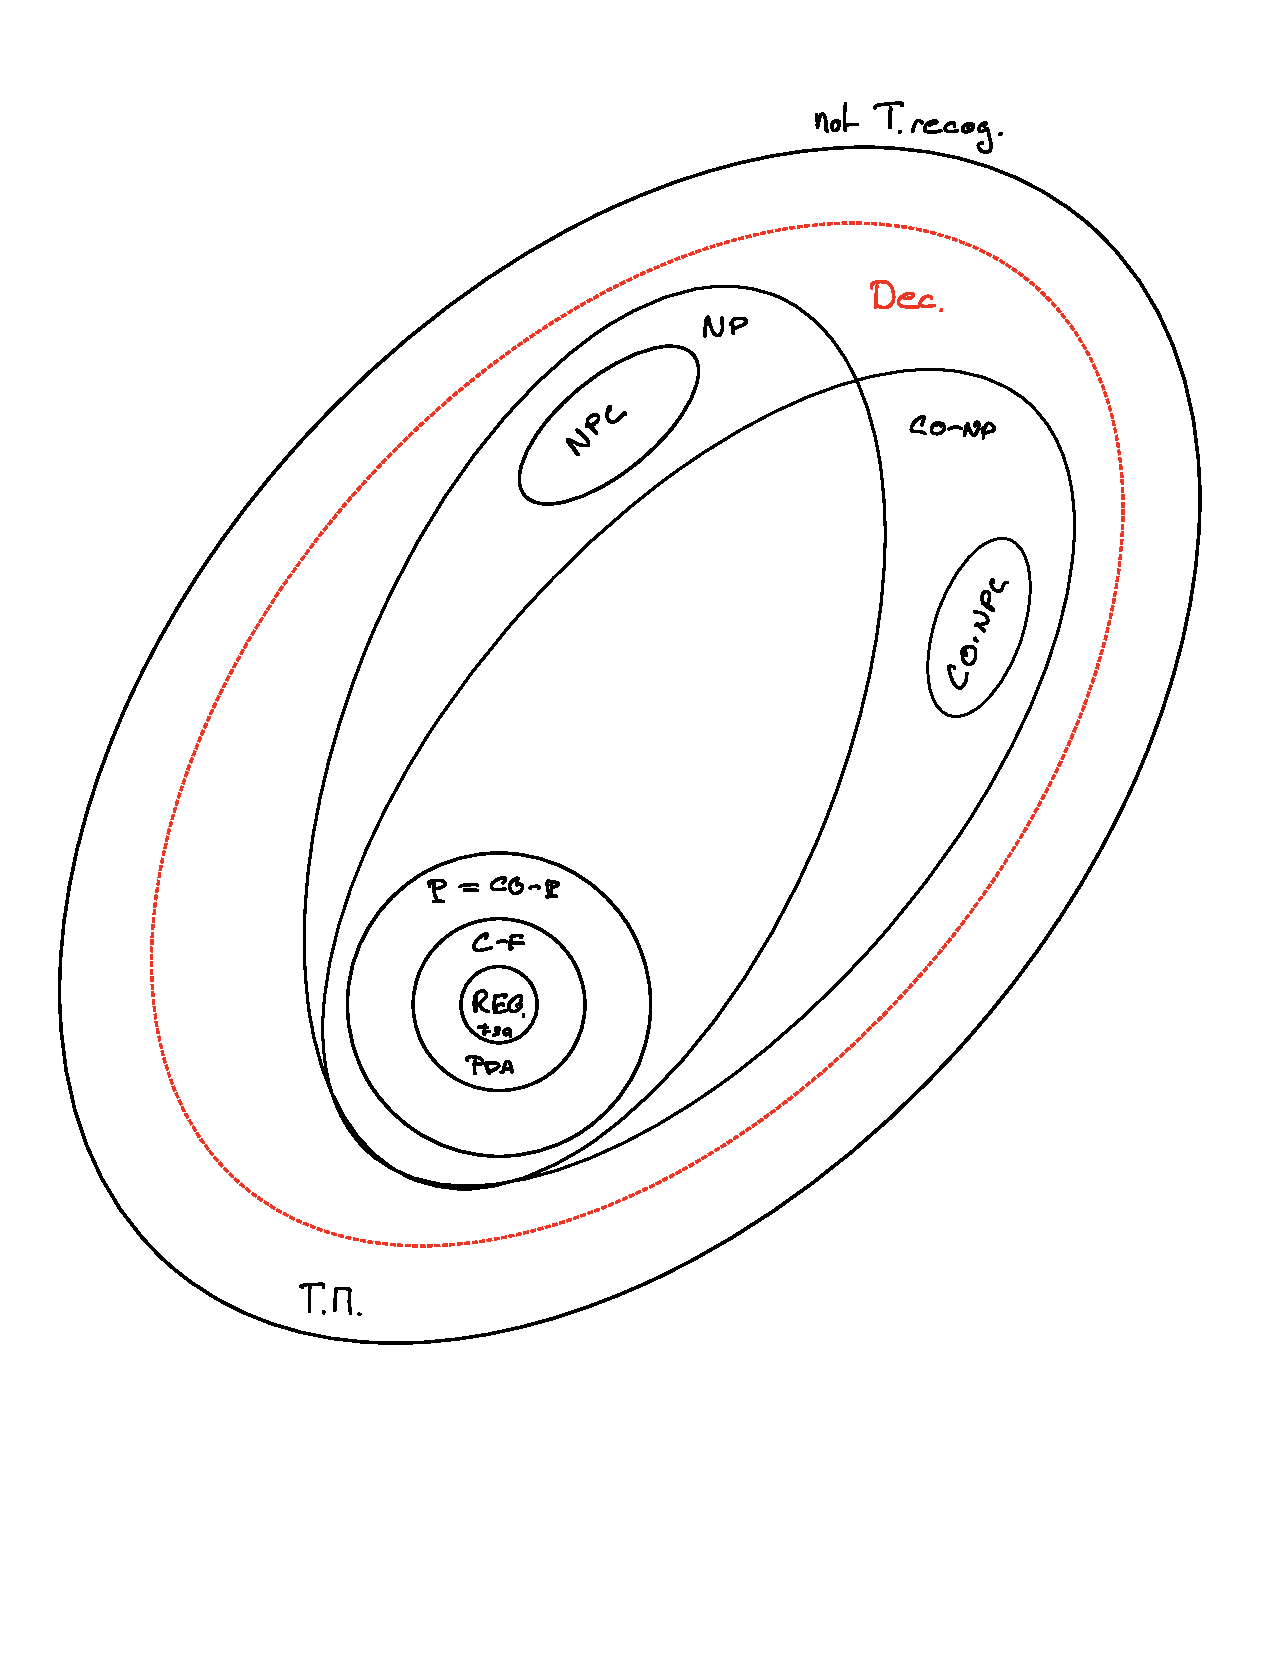
\includegraphics[width=0.95\columnwidth]{assets/conp}

\subsection{NP-Completeness}
\begin{itemize}
  \item $\text{SAT}$: Can a boolean formula (combination of boolean variables and logic variables ($\land, \lor, \lnot$)) be satisfied?
\end{itemize}

\definition{Polynomial Computable Function}{A function $f:\Sigma^*\rightarrow\Sigma^*$, if some polynomial time TM exists that halts with just $f(w)$ on its tape when input $w$.}

\definition{polynomial Time Mapping Reducible}{
  Language $A$ is polynomical time mapping reducible, or simply polynomial time reducible, to language $B$, written $A\le_P B$, if a polynomical time computable function $f: \Sigma^*\rightarrow\Sigma^*$ exists, where for every $w$,
  $$
    w\in A\Longleftrightarrow f(w)\in B.
  $$
}
$f$ is the polynomial time reduction of $A$ to $B$.
\begin{itemize}
  \item If $A\le_P B$ and $B\in \text{P}$, then $A\in\text{P}$
\end{itemize}

\paragraph{\texorpdfstring{$\text{3SAT}$ to $\text{CLIQUE}$}{3SAT to CLIQUE}}
A literal is a boolean variable $x$ or its negation $\overline{x}$. A clause is several literals connected with $\lor$s (e.g. $x_1\lor\overline{x_2}\lor\overline{x_3}$). A conjunctive normal boolean formula (\textbf{cnf-formula}) is composed of several clauses connected with $\land$s. A \textbf{3ncf-formula} is a cnf-formula that has always combines three literals ($(x_1\lor\overline{x_2}\lor x_3)\land(x_4\lor x_5\lor\overline{x_6})$)
\begin{itemize}
  \item $\text{3SAT}=\{\langle\phi\rangle|\phi\text{ is a satisfiable 3cnf-formula.}\}$
\end{itemize}
Reduce $\text{3SAT}$ to $\text{CLIQUE}$: Create a graph with nodes for each literal, no edge between literals of the same clause and between $x_2$ and $\overline{x_2}$, all others are connected. Turns out there is a $k$-clique where $k$ corresponds to the number of clauses in $\phi$. This is because there is at least one true literal in each clause of a satisfied cnf-formula. If the formula is not satisfiable, then there is a contradiction, but no contradictory literals are connected.

\paragraph{\texorpdfstring{$\text{SAT}$ to $\text{SAT-CNF}$}{SAT to SAT-CNF}}
See references.

\paragraph{\texorpdfstring{$\text{SAT-CNF}$ to $\text{3SAT}$}{SAT-CNF to 3SAT}}
\begin{enumerate}
  \item Clause with 2 literals: $x\lor y=(x\lor y\lor u)\land(x\lor y\lor\overline{u})$
  \item 1: $(x)=(x\lor u\lor v)\land(x\lor u\lor\overline{v})\land(x\lor\overline{u}\lor v)\land(x\lor\overline{u}\lor\overline{v})$
  \item k: $(x_1\lor\ldots\lor x_k)=(x_1\lor x_2\lor u_1)\land(\overline{u_1}\lor x_3\lor u_2)\land\ldots\land(\overline{u_{k-4}}\lor x_{k-2}\lor u_{k-3})\land(\overline{u_{k-3}}\lor x_{k-1}\lor x_k)$ (slides: $\overline{x_k}$)
\end{enumerate}


\definition{NP-Completeness}{
  A language $B$ is NP-complete if
  \begin{enumerate}
    \item $B$ is in NP
    \item Every $A\in\text{NP}$ is pol. time reducible to $B$
  \end{enumerate}
}
\begin{itemize}
  \item If $B$ is NP-complete and $B\in\text{P}$, then P=NP.
  \item If $B$ is NP-complete and $B\le_P C$ for $C$ in NP, then $C$ is NP-complete.
\end{itemize}


\begin{center}
  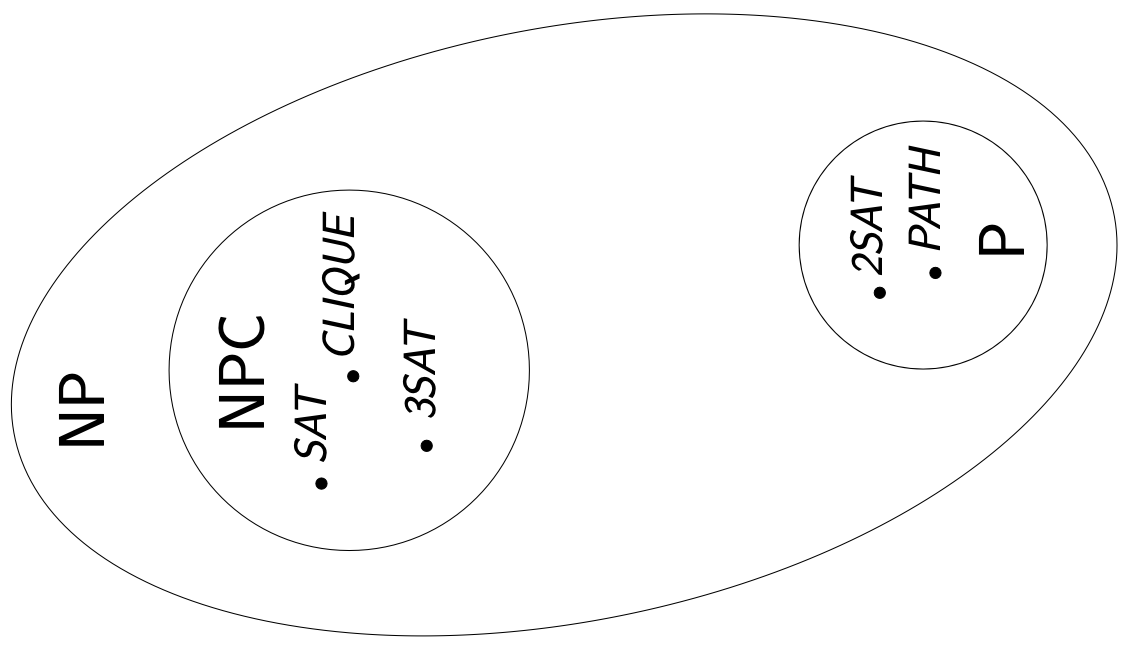
\includegraphics[width=0.75\columnwidth]{assets/npc.png}
\end{center}


\end{document}